\chapter{Implementasi dan Pengujian}

Pada bab ini akan dijelaskan mengenai implementasi, pengujian, dan masalah yang dihadapi. 

\section{Implementasi}
Aplikasi dikembangkan dengan Android Studio, dengan sebuah \textit{laptop} . Aplikasi dijalankan pada x buah ponsel Android.

\subsection{Lingkunan Implementasi}
Berikut adalah spesifikasi \textit{laptop} dan kakas yang digunakan untuk implementasi:

\begin{enumerate}
	\item \textit{Processor} : Intel(R) Core(TM) i7-7700HQ CPU @ 2.80GHz.
	
	\item RAM : 16.0 GB (15.9 GB usable).
	
	\item Versi Android Studio : 4.1.1
	
	\item Google VR for Android : 1.190
\end{enumerate}

Berikut adalah spesifikasi ponsel Android yang digunakan untuk implementasi:

\begin{enumerate}
	\item Processor : Qualcomm Snapdragon 835
	
	\item Sistem Operasi : Android 9.0 (Pie)
	
	\item Sensor yang dimiliki : Accelerometer, gyroscope, magnetometer, step detector.  
\end{enumerate}

\subsection{Hasil Implementasi}
Yang dihasilkan dari implementasi ini adalah aplikasi VR untuk berlari. Aplikasi dapat diperoleh di Google Play Store dan dapat di-\textit{install} pada gawai dengan sistem operasi Android. 

\subsubsection{Tampilan ketika Tombol Ditekan dengan \textit{Textbox} dalam Keadaan Kosong}
Ketika pengguna menekan tombol "\textit{Start Running}" dan keadaan salah satu \textit{textbox} kosong, akan ada \textit{Toast} yang memberikan pesan bahwa \textit{textbox} tidak boleh ada dalam keadaan kosong. Gambar \ref{fig:main-page} menunjukkan tampilah \textit{activity} ini.

\begin{figure}
\centering
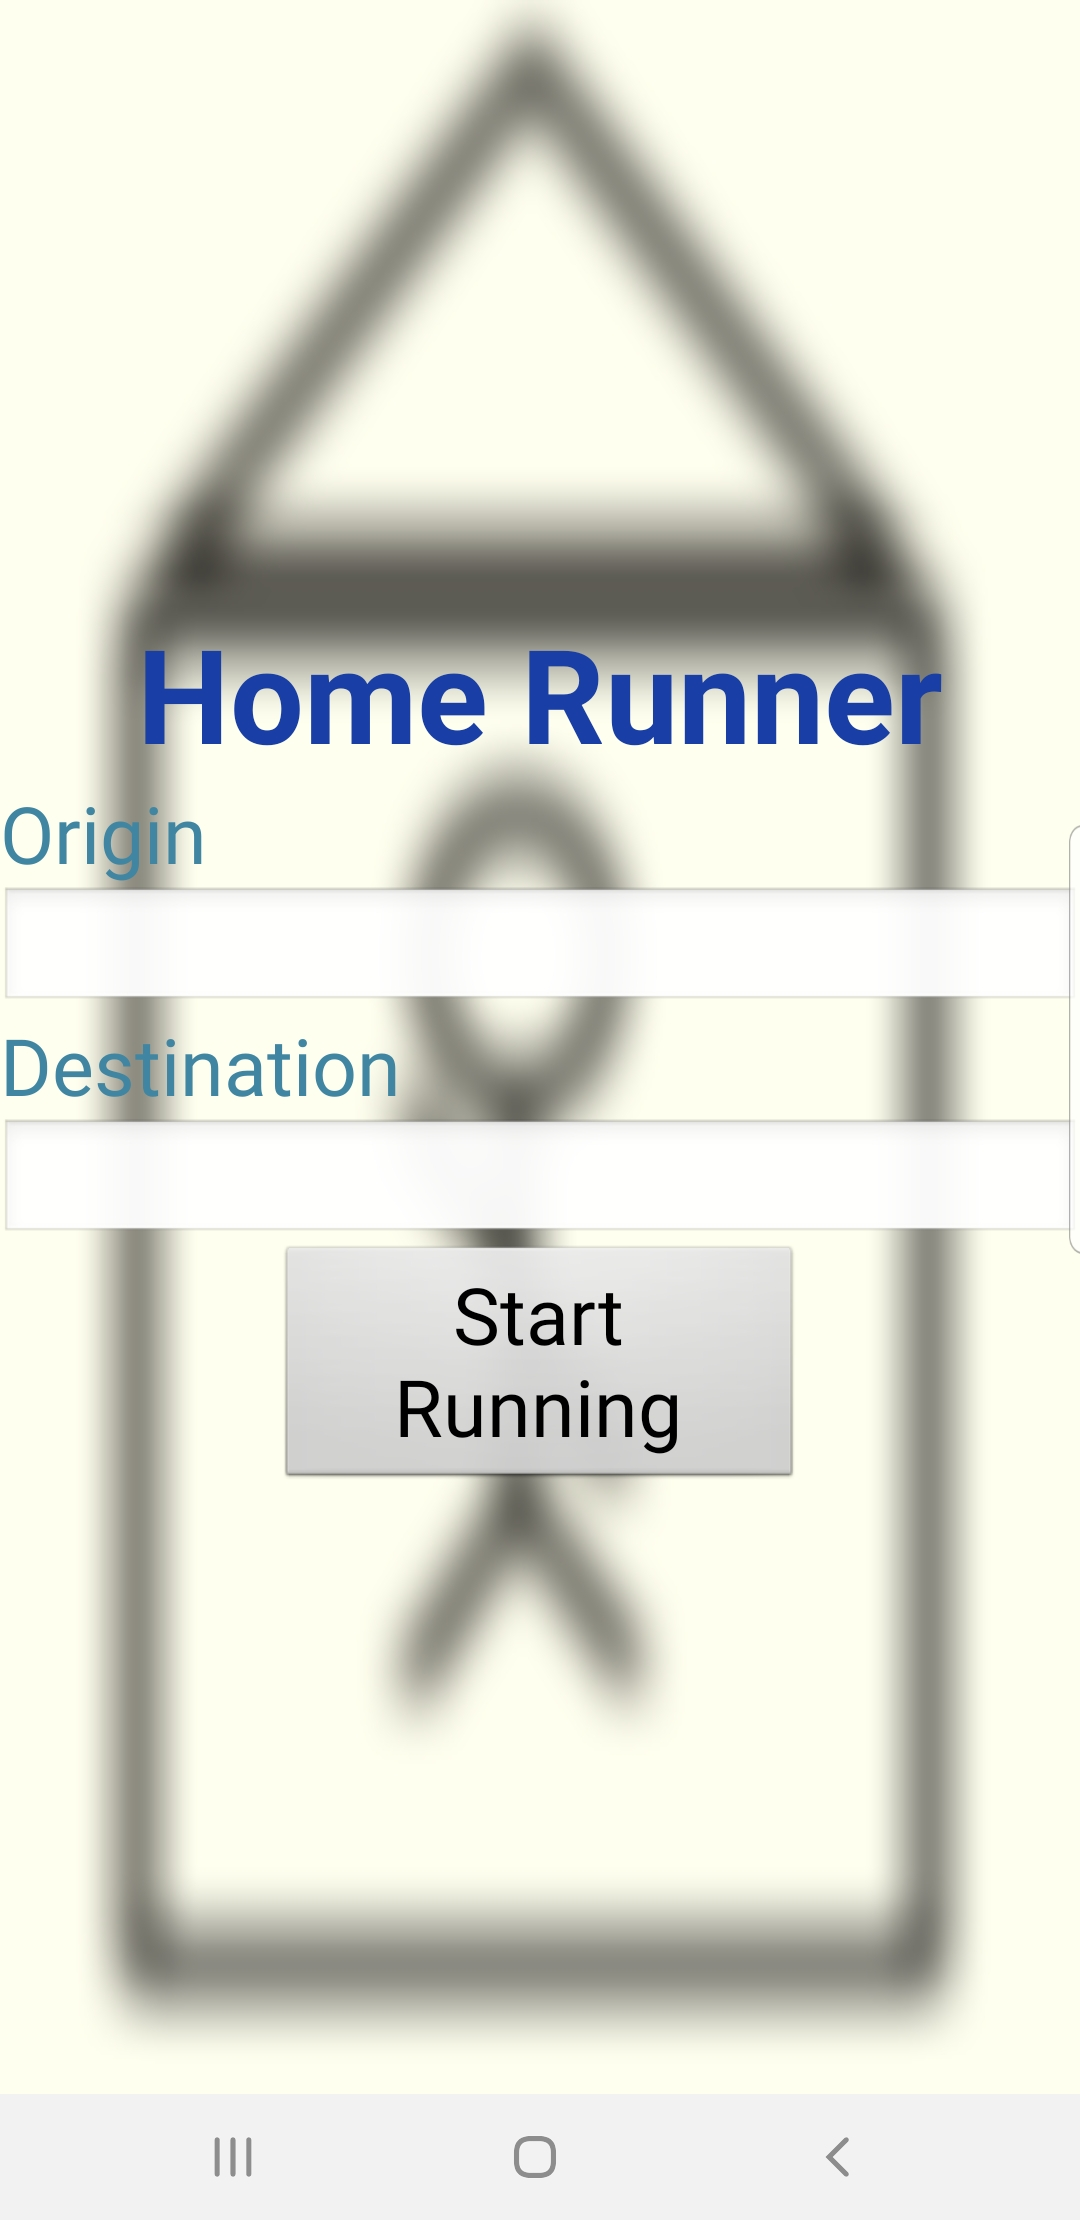
\includegraphics[scale=0.2]{Gambar/main-page.png}
    \caption{\textit{Activity} utama aplikasi}\label{fig:main-page}
\end{figure}

\subsubsection{Aplikasi ketika Masukan Lokasi yang Sah Dimasuukkan, Saat Gawai dalam Posisi \textit{Portrait}}
Saat masukan yang sah dimasukkan pengguna, pengguna akan langsung diarahkan ke halaman yang memberitahu untuk mempersiapkan \textit{Cardboard viewer}, memutar gawai agar menjadi \textit{landscape}. Gambar \ref{fig:cardboard-page} menunjukkan tampilan peringatan ini.

\begin{figure}
\centering
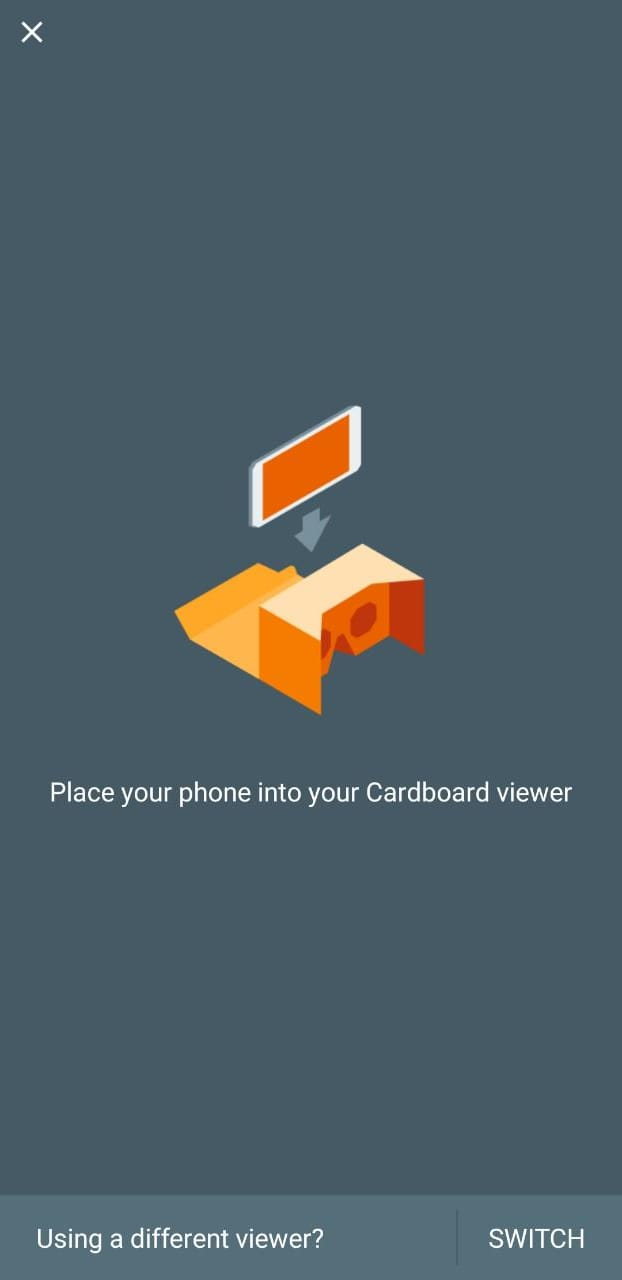
\includegraphics[scale=0.3]{Gambar/cardboard-page.png}
    \caption{Tampilan \textit{Google Cardboard} sebelum gawai diputar}
    \label{fig:cardboard-page}
\end{figure}

\subsubsection{Aplikasi saat Pengguna Berlari}
Setelah memasukkan masukan lokasi asal dan tujuan yang benar lewat dua \textit{textbox}, siap dengan \textit{Cardboard viewer} dan gawai berada dalam posisi \textit{landscape},  aplikasi akan menampilkan dunia VR dengan pemandangan sesuai dengan lokasi asal, dan pemandangan akan berubah sesuai langkah kaki pengguna. \textit{Activity} VR saat pengguna berlari digambarkan pada Gambar \ref{fig:vr-page}.

\begin{figure}
\centering
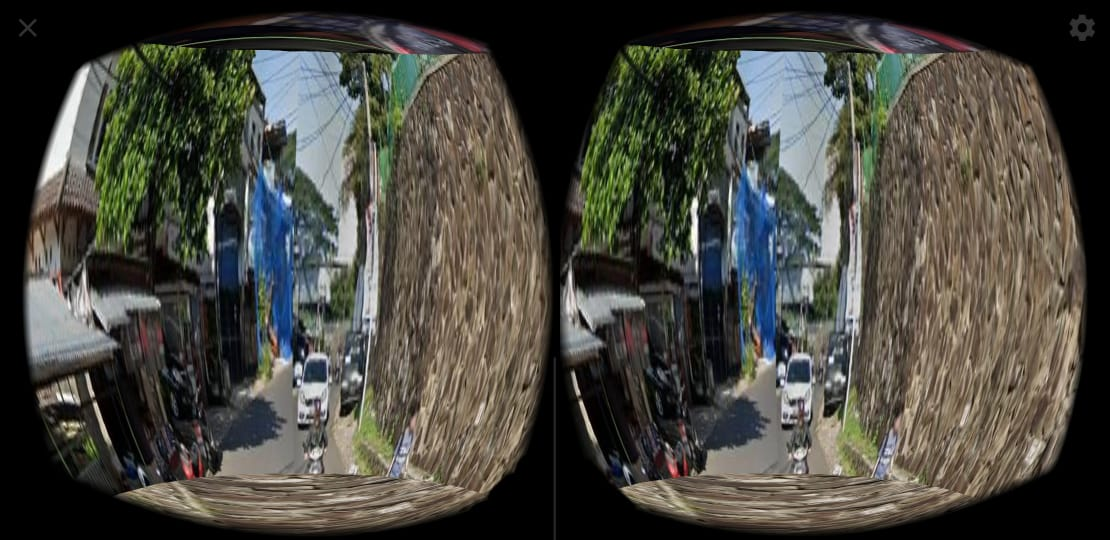
\includegraphics[width=\textwidth]{Gambar/vr-page.png}
    \caption{Tampilan VR saat Pengguna Berlari}
    \label{fig:vr-page}
\end{figure}


\section{Pengujian}



\section{Masalah yang Dihadapi}
Adapun masalah-masalah yang dihadapi dalam proses pengembangan aplikasi adalah sebagai berikut:

\begin{enumerate}
	\item Munculnya galat pada saat mencoba menggambar ulang bangun ruang silinder dengan tekstur baru. Galat tersebut adalah pemanggilan \textit{OpenGL renderer} pada \textit{thread} yang tidak memiliki \textit{context}. 
	
	\item Galat saat meng-\textit{update} Gradle yang membuat kemajuan pengembangan aplikasi terhambat.
\end{enumerate}

